\begin{multicols}{3}[\section{D-Netz}]

\rhead{Tizian Kurkamp, Lucas Heuser}
\lfoot{18.05.2016}

\newrefsegment

\begin{tabular}{p{2,1 cm}p{2.7 cm}}
\textbf{Steckbrief}& \\
\end{tabular}
\rowcolors{1}{\topicolor!20}{}
\begin{tabular}{p{2,1 cm}p{2.7 cm}}
      Einsatz seit & 01.07.1992 \\
	  Eingestellt am & noch in Betrieb\\
      Frequenz"-bereich  & \SI{890} - \SI{960}{\mega\hertz} \\
      Verbreitung & international \\
      Modulation & Frequenzumtastung (GMSK) \\
      Sendeleistung & Feststation: \newline max. \SI{50} Watt \newline
				      Teilnehmer: \newline max. \SI{14} Watt \\
	  Bandbreite eines Kanals & \SI{200}{\kilo\hertz}\\
\end{tabular}
\par
%Source http://www.fh-bingen.de/fileadmin/user_upload/Lehrende/Kilsch_Dieter/internet/projekte/TedoSchStiUnits.pdf -> Seite 9 findet ihr alle verwendbaren Einheiten, wie:
%\SI{Zahl}{\mega\hertz} oder \SI{Zahl}{\mili\metre}
%Ich weiß ehrlich gesagt nicht welche Einheiten ihr im Text genau braucht, aber in dem Dokument und mit obigen Beispiel sollte es umsetzbar ein.


\subsection*{Überblick}
Das D-Netz ist ein zellulares Mobilfunknetz nach dem \textbf{GSM}-Standard (\textbf{G}lobal \textbf{S}ystem for \textbf{M}obile Communications). Die Namensgebung durch den Buchstaben D erfolgt in Fortsetzung der bisherigen Buchstabenbezeichnungen für  vorhergehenden Funknetze (A-, B- und C-Netz).
Das D-Netz ist digitalisiert, sowohl was die Wählvermittlung (Signalling) anbelangt, als auch für Übertragung von Daten und Sprache. Letztere werden quantisiert, digitalisiert und pulscodemoduliert, wodurch sie störungsarm und regenerierbar sind und somit auch unter schwierigen Bedingungen übertragen werden können. Ein besonderes Kennzeichen dieses Zellularnetzes ist der automatische Handover bei einem Wechsel zwischen Funkzellen und das automatische Auffinden von Teilnehmern, deren Standort nicht bekannt ist. Dies ist selbst dann möglich, wenn derzeit kein Gespräch geführt wird und ebenso keine Datenverbindung besteht.

\subsubsection*{Namensgebung und Abgrenzung}
Unter dem Namen D-Netz (oder auch DNetz) werden gleich zwei Netze zusammengefasst. Sowohl die \textit{Telekom} (D1) als auch \textit{Vodafone} nutzen D-Netz Frequenzen um ihre Mobilfunk-Dienste abzuwickeln. Das D-Netz stand ursprünglich für ein digitales Netz im GSM-900-Frequenzbereich und wurde dann später durch das E-Netz (genutzt von \textit{E-Plus} und \textit{o2}) erweitert. Die Namen D1-Netz (für das Netz der \textit{Telekom} bzw. \textit{T-Mobile}) und D2-Netz (für das Netz von \textit{Vodafone}) leiten sich noch aus der ursprünglichen Aufteilung ab.
Mittlerweile gibt es mit UMTS-Netzen und LTE-Netzen deutlich mehr Mobilfunk-Netze, welche genutzt werden können. Die Bezeichnungen haben sich aber mittlerweile so eingebürgert, dass auch ohne die eigentlich vorhandene Netz-Grundlage viele Nutzer diese Kennungen verwenden.



\subsection*{Technische Erläuterung}
Die Übertragung findet im 900-MHz-Bereich statt, und zwar in den Teilbereichen 890 MHz bis 915 MHz und 935 MHz bis 960 MHz. Der untere Frequenzbereich wird für die Übertragung vom Mobilfunk-Sender/Empfänger zur Basisstation genutzt (Uplink). Der obere Bereich entsprechend für die entgegengesetzte Richtung (Downlink). Die Mobilstation wird mit Handy bezeichnet und hat eine Sendeleistung von 0,8 W bis 5 W. Die jeweils 25 MHz breiten Frequenzbereiche sind in 124 Kanäle unterteilt, von denen jeder 200 kHz breit ist. Zur Modulation wird das Frequenzumtastungsverfahren \textbf{GMSK} (\textbf{G}aussian \textbf{M}inimum \textbf{S}hift \textbf{K}eying) verwendet. Hierbei handelt es sich um ein Umtastverfahren, welches zur Übertragung von digitalen Signalen über ein Funkmedium dient. Bei dem GSMK-Verfahren handelt es sich prinzipiell um das Umtastverfahren \textbf{MSK} (\textbf{M}inimum \textbf{S}hift \textbf{K}eying), welches durch einen vorgeschalteten Gauß-Filter ergänzt wird. ~\cite{DNetz.7}     

\begin{Figure}
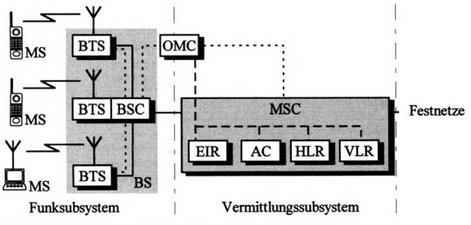
\includegraphics[width=\linewidth]{Kapitel/DNetz/Grafiken/systemaufbau.png}
\captionof{figure}{Systemaufbau des D-Netzes~\cite{DNetz.2}}
\label{fig:DNetz.systemaufbau}
\end{Figure}

Wie auf Abb. \ref{fig:DNetz.systemaufbau} zu sehen ist, besteht das D-Netz aus folgenden Komponenten: 

\begin{itemize}
	\item \textbf{MS} (\textbf{M}obile \textbf{S}tationen)
	\item \textbf{BS} (\textbf{B}asis \textbf{S}tationen) unterteilt in:
		\begin{itemize}
			\item \textbf{BTS} (\textbf{B}ase \textbf{T}ransceiver \textbf{S}tation)
			\item \textbf{BSC} (\textbf{B}ase \textbf{S}tation \textbf{C}ontroller)
		\end{itemize}
	\item \textbf{MSC} (\textbf{M}obile Service \textbf{S}witching \textbf{C}enter) \\ mit je einer: 
		\begin{itemize}
			\item Besucherdatei/\textbf{VLR} \\ (\textbf{V}isitor \textbf{L}ocation \textbf{R}egister)
			\item Heimatdatei/\textbf{HLR} \\ (\textbf{H}ome \textbf{L}ocation \textbf{R}egister)
			\item Authentifizierungszentrale/\textbf{AC} \\ (\textbf{A}uthentification \textbf{C}enter)
			\item Endgerätkennungsdatei/\textbf{EIR} \\ (\textbf{E}quipment \textbf{I}dentity \textbf{R}egister)
		\end{itemize}
	\item Zentrale Betriebstechnik/\textbf{OMC} \\ (\textbf{O}peration and \textbf{M}aintenance \textbf{C}enter) \\
\end{itemize}


Hierbei stellen MS im generellen Fall ein Funktelefongerät dar. Es kann sich allerdings prinzipiell um ein beliebiges D-Netz-kompatibles Endgerät handeln (z.B. einen Laptop mit Sende und Empfangseinheit). Diese MS kommunizieren mit den BTS, welche als reine Funksende- und Empfangsmodule dienen. Verschiedene MS sind widerrum an einen BSC gekoppelt welcher die Kommunikationen koordiniert und an das Funkvermittlungssystem, also das MSC, weiterleitet. Die Funkvermittlung an sich besteht wie in der Übersicht schon zu sehen ist aus diversen Komponenten, welche alle eine spezifische Aufgabe innerhalb der Vermittlung durchführen. Die Besucherdatei VLR ist eine Datenbank, in welcher diverse Informationen zu allen Teilnehmern einer MS abgelegt werden, welche nötig sind um eine korrekte Gesprächsverbindung aufbauen zu können ~\cite{DNetz.8}. Die HLR-Datenbank beinhaltet Informationen zu Teilnehmern, welche einem bestimmten stationären Bereich zuzuordnen sind. Das jeweilige HLR-Register kann im Falle von Roaming durch die Teilnehmerrufnummer ermittelt werden, womit das dynamische Aktualisieren der VLR-Daten durch das HLR ermöglicht wird ~\cite{DNetz.9}. Die nächste Komponenten, das AC, dient zur korrekten Authentifizierung eines Teilnehmers an Hand seiner verwendeten \textbf{SIM}-Karte (\textbf{S}ubscriber \textbf{I}dentity \textbf{M}odule) innerhalb des Mobilfunknetzes. Die Gerätedatenbank (EIR) wird dazu verwendet die \textbf{IMEI}-Nummer (\textbf{I}nternational \textbf{M}obile \textbf{E}quipment \textbf{I}dentitie) aller an einer BS registrierten MS zu überprüfen und bei Fehlern (defekte oder modifizierte Geräte) oder gestohlenen Geräten die Verbindungen dieses Teilnehmers zu unterbinden ~\cite{DNetz.10}. Die IMEI-Nummer ist eine 15-stellige und theoretisch eindeutige Identifikationsnummer, welche jegliches GSM- oder UMTS-Engerät weltweit identifizieren kann. In Abb. \ref{fig:DNetz.imei} ist der vereinfachte Aufbau einer IMEI-Nummer zu sehen.     

\begin{Figure}
\includegraphics[width=\linewidth]{Kapitel/DNetz/Grafiken/imei.png}
\captionof{figure}{Vereinfachter Aufbau einer IMEI-Nummer}
\label{fig:DNetz.imei}
\end{Figure}

Obwohl die IMEI-Nummer per Definition eine eindeutige und gerätespezifische Identifikationsnummer ist, kommt es in der Praxis durchaus vor, dass mit Hilfe manipulierter Endgeräte eine falsche IMEI-Nummer vorgetäuscht werden kann. Verantwortlich für den Schutz vor Manipulationen und die Einhaltung der Richtlinien sind die Gerätehersteller selbst.~\cite{DNetz.11}




\subsection*{Einsatz}
Da das D-Netz auf auf dem GSM-900-Standart beruht, steht es in vielen Staaten weltweit zur Verfügung. Durch diverse Roamingabkommen wird es den Teilnehmern ermöglicht, die MS grenzüberschreitend in mehr als 130 Ländern zu verwenden. In Deutschland wird das D-Netz als Nachfolger des B-Netzes, welches im Jahre 2000 offiziell eingestellt wurde, verwendet und von der \textit{Deutschen Telekom} und \textit{Vodafon} verwaltet. 




\subsection*{Anbieter und Gremien}
Für das D-Netz gibt es in Deutschland zwei Betreiber: Die \textit{Telekom}, welche das D1-Netz zur Verfügung stellt und \textit{Vodafone} mit dem D2-Netz. Da beide Netze nach dem GSM-Standard betrieben werden, gibt es technisch kaum Unterschiede. Damit man allerdings die beiden Betreiber an den Rufnummern unterscheiden kann, sind die Netzkennzahlen unterschiedlich.

Einige Anbieter im D1-Netz (\textit{Telekom}) sind:

\begin{itemize}
\item \textit{Deutsche Telekom}
\item \textit{congstar}
\item \textit{freenetmobile}
\item \textit{ja!mobil}
\item \textit{Penny Mobil}
\end{itemize}
und noch Weitere mehr. \newline

Einige Anbieter im D2-Netz (\textit{Vodafon}) sind:

\begin{itemize}
\item \textit{Vodafone}
\item \textit{1und1}
\item \textit{callmobile.de}
\item \textit{FYVE}
\item \textit{klarmobil}
\end{itemize}
und noch Weitere mehr.
(Vgl. ~\cite{DNetz.1})




\end{multicols}
\newpage
\section*{Historische Entwicklung}
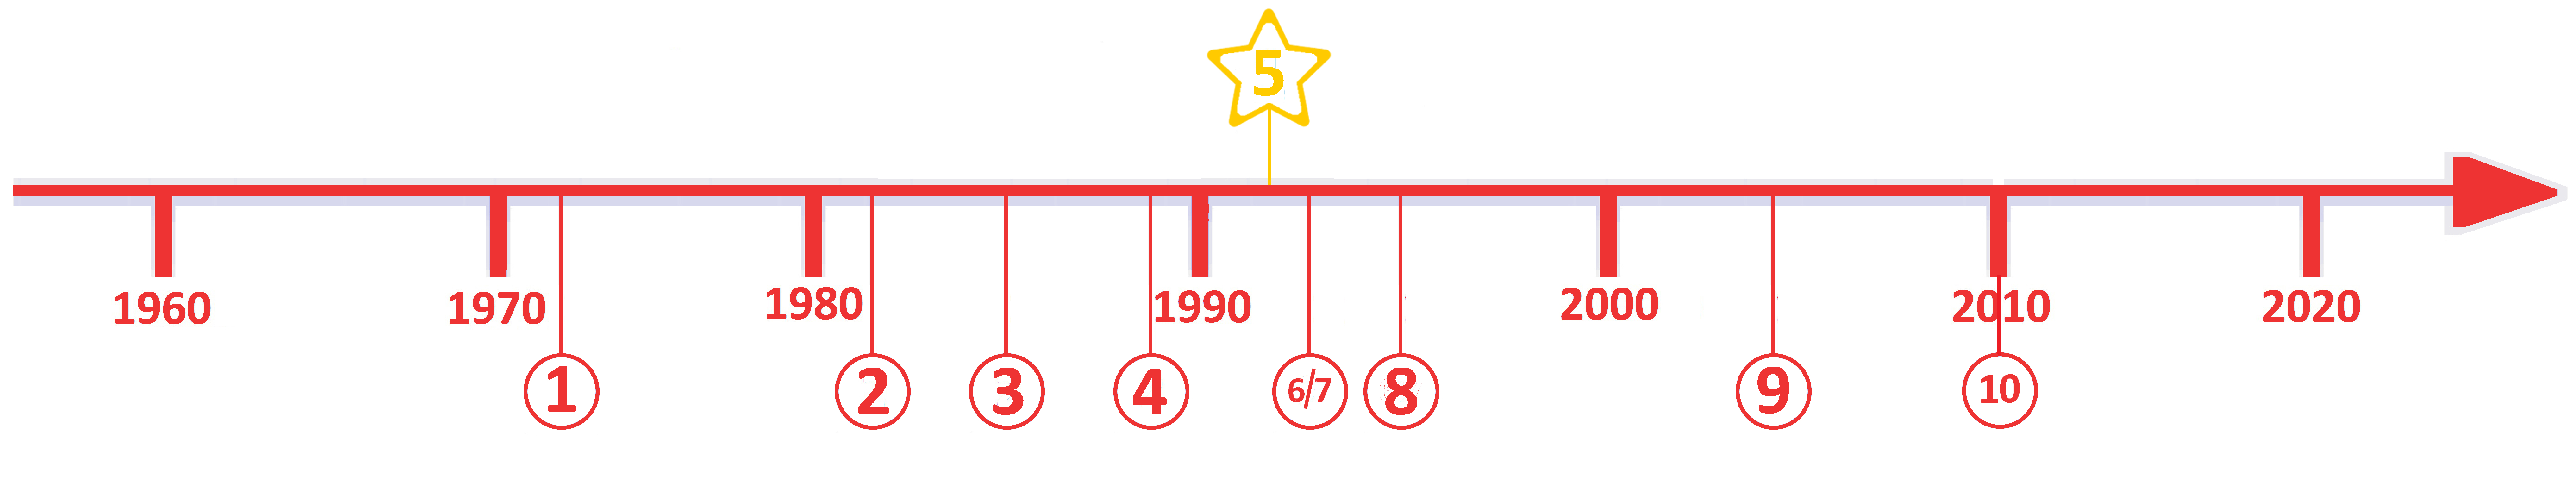
\includegraphics[width=\textwidth]{Kapitel/DNetz/Grafiken/zeitstrahl.png}
\par
\noindent
\rowcolors{2}{}{\topicolor!20}
\begin{tabular}{p{0.5 cm}p{1.5 cm}p{15.55 cm}}
	Nr. & Datum & Entwicklungsschritte ~\cite{c-netz.7} \\
	1 & 1972 & Realisierung des B-Netzes \\
	2 & 1982 & Gründung der \textit{\textbf{GSM}} (damals: \textit{\textbf{G}roupe \textbf{S}pécial \textbf{M}obile})\\
	3 & 1985 & Einführung des C-Netzes \\
	4 & 07.12.1989 & Vergabe einer Lizenz an ein Konsortium unter der Führung des \textit{Mannesmann-Konzerns} \\
	5 & 01.07.1992 & Start des Regelbetriebs des D-Netzes \\
	6 & April 1993 & ca. 130.000 Netz-Teilnehmer bei der \textit{Telekom} \\
	7 & Ende 1993 & 80\%ige Abdeckung Deutschlands durch das D2-Netz \\
	8 & 1994/95 &  Einführung des \textit{E-Plus}-Mobilfunknetzes \\
	9  & 2004 &  ca. 71 Millionen Mobilfunknutzer und Einführung des UMTS-Netzes \\
	10 & 2010 & Einführung des LTE-Mobilfunkstandards \\
\end{tabular}
\par
\begin{multicols}{3}


\begin{wrapfigure}{r}{0.4\linewidth}
  \vspace{-1pt}
  \begin{center}
  	\hspace{-20pt}
    
\includegraphics[width=0.7\linewidth]{Kapitel/DNetz/Grafiken/gsm_logo.png}
  \end{center}
  \vspace{-10pt}
\end{wrapfigure}
1982 wurde die \textit{Groupe Spéciale Mobile} gegründet, welche für Europa ein einheitliches digitales Mobilfunksystem entwickeln sollte. Als sich Ende der 1980er Jahre die praktische Umsetzung des Standards abzeichnete, wurde in Deutschland vom Postminister Christian Schwarz-Schilling entschieden, dass neben der \textit{Bundespost} auch ein privater Anbieter eine Lizenz für den Betrieb eines Netzes des GSM-Standards erhalten sollte. In dem Ausschreibungsverfahren wurde festgelegt, dass zwischen beiden Betreibern faire Wettbewerbsbedingungen bestehen sollten. Insgesamt zehn Firmen bewarben sich um die Lizenz, die am 7. Dezember 1989 schließlich an ein Konsortium unter Führung des \textit{Mannesmann-Konzerns} vergeben wurde, da dieser nach Meinung des Lenkungsausschusses Mobilfunk den leistungsfähigsten Bewerber darstellte.
Nach einer einjährigen Versuchsphase wurde der Regelbetrieb am 1. Juli 1992 gestartet. Als unmittelbarer Nachfolger des C-Netzes erhielt das neue Netz die Bezeichnung „D-Netz“.
Das D1-Netz ist das Netz der \textit{Deutschen Telekom}, während das D2-Netz das Mobilfunknetz der Firma \textit{Vodafon} bezeichnet, ehemals Mannesmann Mobilfunk. Nach der Einführung des \textit{E-Plus}-Mobilfunknetzes 1994 setzte ein erheblicher Preisfall bei den Endgeräten, sowie bei der Tarifstruktur ein, sodass die Teilnehmerzahl rapide anstieg.(Vgl. ~\cite{DNetz.3} und ~\cite{DNetz.4})




\subsection*{Ausblick}
Als das Handy sich in den 1990er-Jahren in Deutschland etablierte, war Mobilfunk noch etwas Besonderes und die Nutzung von Handys vorwiegend auf das Telefonieren und SMS-Schreiben beschränkt. Auch die Netzabdeckung steckte in Deutschland noch in den Kinderschuhen. Heute gehört das Smartphone mit seinen vielseitigen Funktionen zum Standard des modernen Menschen. Mobiles surfen, telefonieren, chatten oder Bilder versenden ist, dank moderner Mobilfunknetze, problemlos auch von unterwegs möglich. Vor allem der neue Standard LTE verspricht Internetgeschwindigkeiten, wie man sie bisher nur von DSL im Heimbereich gewohnt war.
Die vier großen Mobilfunkbetreiber, die \textit{Telekom}, \textit{o2}, \textit{Vodafone} und \textit{E-Plus} kommen in Deutschland auf eine nahezu vollständige GSM-Netzabdeckung. Somit sollte man mit nahezu jedem Anbieter fast überall in Deutschland problemlos telefonieren oder eine Kurznachricht versenden können. In Deutschland haben wir also im GSM-Netz eine Netzabdeckung von nahezu 100 Prozent! Allerdings zeigt es sich in der Praxis des Öfteren, dass in manchen Gebieten beim Telefonieren Funklöcher entstehen können. Ebenso gibt es weitere Unterschiede bezüglich der Netzabdeckung mit verschiedenen Übertragungsarten wie \textbf{UMTS} (\textbf{U}niversal \textbf{M}obile \textbf{T}elecommunications \textbf{S}ystem) oder \textbf{LTE} (\textbf{L}ong \textbf{T}erm \textbf{E}volution).

Schnelle Übertragungsraten sind theoretisch auch heute schon per LTE Advanced möglich. Die zukünftige Entwicklung der Mobilfunkstandards wird demnach nicht allein von der bereits erreichten Bandbreite, sondern noch viel stärker davon abhängen, wie gut die Netze ausgebaut werden, damit auch das gesamte Leistungsspektrum genutzt werden kann.

Ein wichtiger Motor für den Ausbau der Mobilfunkstandards ist unter anderem auch der Mobile Commerce, als Teil des E-Commerce. Denn immer mehr Menschen kaufen auch mit ihrem Tablet oder Smartphone im Internet ein. Durch den flächendeckenden Ausbau des LTE-Netzes ist es dann auch möglich, überall und jederzeit in Deutschland online einzukaufen. Auch die Internetnutzung allgemein wird LTE verändern, denn bei voller Netzabdeckung wäre niemand mehr in Deutschland auf einen Festnetzanschluss angewiesen, um schnelles Internet zu nutzen. Vielleicht werden dann in Zukunft auch Festnetzanschlüsse obsolet?

LTE ist zukunftsweisend, der Netzausbau des mobilen Internets wird voraussichtlich den Ausbau des DSL-Netzes in Deutschland übertreffen. Für Bewohner in ländlichen Regionen wäre dies zukünftig eine gute Nachricht, denn sie sind bis dato immer noch vom schnellen Breitbandinternet abgeschnitten.

\printbibliography[segment=5,heading=subbibliography]
\end{multicols}
\newpage
